% This is "sig-alternate.tex" V2.0 May 2012
% This file should be compiled with V2.5 of "sig-alternate.cls" May 2012
%
% For tracking purposes - this is V2.0 - May 2012

\documentclass{sig-alternate}
\usepackage{graphicx}
\usepackage{subfigure}
\usepackage{url}
\usepackage{indentfirst}
\usepackage{cite}


\usepackage{color}
\newcommand{\red}[1]{\textcolor{red}{#1}}
\newcommand{\blue}[1]{\textcolor{blue}{#1}}



\usepackage[normalem]{ulem}


\begin{document}
%
% --- Author Metadata here ---
\conferenceinfo{WOODSTOCK}{'97 El Paso, Texas USA}
%\CopyrightYear{2007} % Allows default copyright year (20XX) to be over-ridden - IF NEED BE.
%\crdata{0-12345-67-8/90/01}  % Allows default copyright data (0-89791-88-6/97/05) to be over-ridden - IF NEED BE.
% --- End of Author Metadata ---

\title{Temporal Evolution of Scientific Communities
\titlenote{(Produces the permission block, and copyright information). For use with SIG-ALTERNATE.CLS. Supported by ACM.}}
\subtitle{[Deadline February 22, 2013]
\titlenote{A full version of this paper is available as \textit{Author's Guide to Preparing ACM SIG Proceedings Using
\LaTeX$2_\epsilon$\ and BibTeX} at
\texttt{www.acm.org/eaddress.htm}}}
%
% You need the command \numberofauthors to handle the 'placement
% and alignment' of the authors beneath the title.
%
% For aesthetic reasons, we recommend 'three authors at a time'
% i.e. three 'name/affiliation blocks' be placed beneath the title.
%
% NOTE: You are NOT restricted in how many 'rows' of
% "name/affiliations" may appear. We just ask that you restrict
% the number of 'columns' to three.
%
% Because of the available 'opening page real-estate'
% we ask you to refrain from putting more than six authors
% (two rows with three columns) beneath the article title.
% More than six makes the first-page appear very cluttered indeed.
%
% Use the \alignauthor commands to handle the names
% and affiliations for an 'aesthetic maximum' of six authors.
% Add names, affiliations, addresses for
% the seventh etc. author(s) as the argument for the
% \additionalauthors command.
% These 'additional authors' will be output/set for you
% without further effort on your part as the last section in
% the body of your article BEFORE References or any Appendices.

\numberofauthors{3} %  in this sample file, there are a *total*
% of EIGHT authors. SIX appear on the 'first-page' (for formatting
% reasons) and the remaining two appear in the \additionalauthors section.
%
\author{
% You can go ahead and credit any number of authors here,
% e.g. one 'row of three' or two rows (consisting of one row of three
% and a second row of one, two or three).
%
% The command \alignauthor (no curly braces needed) should
% precede each author name, affiliation/snail-mail address and
% e-mail address. Additionally, tag each line of
% affiliation/address with \affaddr, and tag the
% e-mail address with \email.
%
% 1st. author
\alignauthor Bruno Leite Alves\\
       \affaddr{UFMG}\\
       \affaddr{Belo Horizonte, Brazil}\\
       \email{bruno.leite@dcc.ufmg.br}
% 2nd. author
\alignauthor Fabr\'icio Benevenuto\\
       \affaddr{UFMG}\\
       \affaddr{Belo Horizonte, Brazil}\\
       \email{fabricio@dcc.ufmg.br}
% 3rd. author
\alignauthor Alberto H. F. Laender\\
      \affaddr{UFMG}\\
      \affaddr{Belo Horizonte, Brazil}\\
      \email{laender@dcc.ufmg.br}
}

\maketitle
\begin{abstract}

\end{abstract}

% A category with the (minimum) three required fields
\category{H.4}{Social Network}{Temporal Analisys}
%A category including the fourth, optional field follows...
%\category{D.2.8}{Software Engineering}{Metrics}[complexity measures, performance measures]
\category{J.4.} {Computer Applications} Social and behavioral sciences {Miscellaneous}

\terms{Human Factors, Measurement.}


\keywords{communities, scientific communities, core community, evolution}

\section{Introduction}

Since its beginning, society has been organizing itself into communities, which are groups of people with common interests. Particularly, the proliferation of new communication
technologies based on the Internet has facilitated the rapid formation and growth of online communities. Communities exhibit a wide range of characteristics and serve a variety of
purposes, from small groups engaged in tightly niche topics such as a very specific scientific community, to millions of users linked by an interest such as a community related to
a sport team or fans of a celebrity. 

Often, individuals who are socially connected in a community tend to share interests and similarities. Although, there are many factors that might determine a community formation
and its growth, there are two main driven forces used to explain similarity in a community formation: influence and homophily. On one hand, influence posits that individuals change
to become more similar to their friends in the community. On the other hand, homophily postulates that individuals create social connections within a community precisely because
they are already similar. Recent efforts have provided quantitative evidences of both forces~\cite{icwsm10cha,crandall.kdd08,Backstrom:2006,influence.correlation.kdd08} and several existing
theories~\cite{Rogers.1962,katz1955,accidental-influential}, models~\cite{kempe03kdd,Kempe05influentialnodes}, and
approaches~\cite{saez-trumper@kdd12,Weng:2010:TFT:1718487.1718520} rely on identifying a group of influential individuals with the power to affect not only the underlying network
structure of a community, but also to interfere on the spread and flow of information within a community. 


In this paper, we take a different perspective and study a complementary problem. Here, we focus on studying the roles that community leaders play and how they can impact intrinsic
evolving properties of communities. From a sociological perspective, it helps us understanding how segments of society evolve as well as answering longstanding  questions related
to the interaction among different types of participants. From the computer science perspective, understanding  these aspects is
critical not only for link prediction as well as the designing better recommendation systems, but it is also a necessary step for viral marketing strategies and social campaigns.
Such a study, however, has been difficult as essential components like human connections and a proper definition of leadership is hard to be reproduced at a large scale within the
confines of a research laboratory.

We focus on studying the role of leaderships in scientific communities. When prolific research leaders decide to join or leave communities, they take with them resources,
experience, students and possibly influence other authors to do the same, which makes scientific communities very suitable for this kind of study. We used data from DBLP to identify
scientific communities, represented by the main ACM SIGs conferences. Then, we propose a strategy to infer the community core, the leaders of a given scientific community in a
given period of time. Finally, we investigate how aspects of the core might impact on the community structure. Our results show that… (\red{TO DO}). 

The rest of this paper is organized as follows. Next section surveys related efforts. Then, Section 3 describes our strategy and dataset used to construct the connections around
scientific communities and analyzes the main evolving properties of this communities.  Section 4 describes our strategy to compute the community core and Section 5 investigate the
main properties of these sets of authors within their communities.  Finally, Section 6 concludes the paper and provides directions for future work. 










\section{Related Work}
Studies has been done to understand the structure of social networks, some studies has focus at temporal evolutions. 
In this terms, \cite{Viswanath:2009} shows a studies where they used two Facebook's dataset. 
The first dataset is about user's profile information, in other words, it is just the user's public information 
and friendship. 
The second dataset contains the data of interaction between the user's Facebook. In Facebook, a user's friends 
can post comment's to the user's wall, these comments appear on the user's wall and can be seen  by others who 
visit the user's profile. 
In these way, \cite{Viswanath:2009} modeled the first dataset as a undirectional graph and the second as a directional 
graph to analysis.
\cite{Viswanath:2009} shows that the second dataset contains information about link's disappearance, because user 
usually stopped to interact, but hardly he removes a friendship tie, it is the cause of the first dataset do not have 
this information. Other cause of the first dataset do not represent the real world is that some users just accept a 
friendship invite as courtesy. In this paper also is showed a measures to show the link's evolutions on the time, 
the resemblance.
\cite{Viswanath:2009} showed that, in the second dataset, though there is high churn in the user pairs that interact 
over time, many of the global structural properties remained relatively constant over time.\\
\\
Is showen in another study \cite{Kumar:2006} the components evolutions of two social networks of a big company. These 
study analysis the components of three ways. The analysis is done about nodes that have degree one, intermidiate components 
(components that are not the gigant component and has more than one degree) and the gigant component. In the intermidiate 
components is showed the concept of star nodes, this nodes are importants to the social networks, because they can make 
the social network grow. Also proposed is mathematic model that making the prediciton of behavior identified in these 
study. In this study \cite{Kumar:2006} is done a characterize about the nodes type too where they can be passive, 
linkers and invites.
\\
\cite{Sun:2012} \\
\cite{Ducheneaut:2007} \\
\cite{Backstrom:2006} \\
\cite{Patil:2012} \\
\cite{Lopes:2011} \\
\cite{Sachan:2012} \\
\cite{Leskovec:2005} \\
\cite{Xu:2010} \\
\cite{Willinger:2010} \\
\cite{Wu:2009} \\
\cite{Huang:2008} \\
\cite{Garg:2009} \\
\cite{Leskovec:2008} \\


\section{Scientific Communities}
\subsection{Dataset}
The dataset consists of the digital libary DBLP\footnote{http://dblp.uni-trier.de/}\cite{Ley:2009}. The DBLP is presented as a 
timegraph. We enrich the dataset with some information wich be explained below.\\
The DBLP is a digital libary has more than 2.1 milhon of publications and 
1.2 milhon of authors. The digital libary store many information about the researcher and their works published, 
one of this information is the publication date, being the first entry found in the digital libary dated from 1936.
The DBLP offers its data in XML format, thereby facilitating the use of its data to study. How the publications 
data has the date and coauthoring, we can using the DBLP data to make a temporal coauthoring 
network which the nodes match to authors and the edge between them match to collaborative work with the date,
so it is possible to obtain the state of network at a given time.\\
How DBLP has a lot of data and these data have many types, some conferences were chosen for this study. In order
to avoid any bias and obtain heterogenous data, we choose the flagship conference each ACM SIGs (Special Interest Groups).
The ACM SIGs representing many major area of computing. The SIGs offers a wealth of conferences on the global 
scale, providing unlimited opportunities. In this way, this work uses the data from the DBLP which match the flagship 
conferences of SIGs. We were unable to use all SIGs or some conferences by problems of data crossing, for example,
younger conferences do not have enough data to study or biannual conferences may clash with the other. So, we 
performed an analysis to select conferences with significant amount of data and to be continuous.\\
The Table \ref{tab:sigs_conference_period} shows the conferences chosen, along with relevant information about them.
In the sequence, it is possible to see the SIG, the name of conference, the period used (some conferences have had
it period reduced to maintain the continuity of data), the h-index of the conference (explained in the nexts section),
number of authors, number of publications, number of editions, average of authors per editions, average of publications
per editions and average of authors per publications.

\begin{table*}[!htb]
\centering
\caption{The data of DBLP of flagship conferences of ACM SIGs}
\label{tab:sigs_conference_period}
{\small
\begin{tabular}{|l|l|c|c|c|c|c|c|c|c|} \hline
SIG & Conference & Period & H-Index & Authors & Publications & Editions & Aut/Edi & Pub/Edi & Aut/Pub\\ \hline
SIGACT & STOC & 1969-2012 & 94 & 2159 & 2685 & 44 & 49.07 & 61.02 & 0.80\\ \hline
SIGAPP & SAC & 1993-2011 & 59 & 9146 & 4500 & 19 & 481.37 & 236.84 & 2.03\\ \hline
SIGARCH & ISCA & 1976-2011 & 102 & 2461 & 1352 & 36 & 68.36 & 37.56 & 1.82\\ \hline
SIGBED & HSCC & 1998-2012 & - & 846 & 617 & 15 & 56.40 & 41.13 & 1.37\\ \hline
SIGCHI & CHI & 1994-2012 & 144 & 5095 & 2819 & 19 & 268.16 & 148.37 & 1.81\\ \hline
SIGCOMM & SIGCOMM & 1988-2011 & 140 & 1593 & 796 & 24 & 66.38 & 33.17 & 2.00\\ \hline
SIGCSE & SIGCSE & 1986-2012 & 51 & 3923 & 2801 & 27 & 145.30 & 103.74 & 1.40\\ \hline
SIGDA & DAC & 1964-2011 & 98 & 8876 & 5693 & 48 & 184.92 & 118.60 & 1.56\\ \hline
SIGDOC & SIGDOC & 1989-2010 & 23 & 1071 & 810 & 22 & 48.68 & 36.82 & 1.32\\ \hline
SIGGRAPH & SIGGRAPH & 1985-2003 & 119 & 1920 & 1108 & 19 & 101.05 & 58.32 & 1.73\\ \hline
SIGIR & SIGIR & 1978-2011 & 116 & 3624 & 2687 & 34 & 106.59 & 79.03 & 1.35\\ \hline
SIGKDD & KDD & 1995-2011 & 124 & 3078 & 1699 & 17 & 181.06 & 99.94 & 1.81\\ \hline
SIGMETRICS & SIGMETRICS & 1981-2011 & 71 & 2083 & 1174 & 31 & 67.19 & 37.87 & 1.77\\ \hline
SIGMICRO & MICRO & 1987-2011 & 81 & 1557 & 855 & 25 & 62.28 & 34.20 & 1.82\\ \hline
SIGMM & Multimedia & 1993-2011 & 80 & 5400 & 2928 & 19 & 284.21 & 154.11 & 1.84\\ \hline
SIGMOBILE & MobiCom & 1995-2011 & 106 & 1151 & 480 & 17 & 67.71 & 28.24 & 2.40\\ \hline
SIGMOD & SIGMOD & 1975-2012 & 147 & 4202 & 2669 & 38 & 110.58 & 70.24 & 1.57\\ \hline
SIGOPS & PODC & 1982-2011 & 59 & 1685 & 1403 & 30 & 56.17 & 46.77 & 1.20\\ \hline
SIGPLAN & POPL & 1975-2012 & 85 & 1527 & 1217 & 38 & 40.18 & 32.03 & 1.25\\ \hline
SIGSAC & CCS & 1996-2011 & 97 & 1354 & 676 & 16 & 84.63 & 42.25 & 2.00\\ \hline
SIGSAM & ISSAC & 1988-2011 & - & 1100 & 1177 & 24 & 45.83 & 49.04 & 0.93\\ \hline
SIGSOFT & ICSE & 1987-2011 & 111 & 3502 & 2248 & 25 & 140.08 & 89.92 & 1.56\\ \hline
SIGUCCS & SIGUCCS & 1989-2011 & - & 1771 & 1593 & 23 & 77.00 & 69.26 & 1.11\\ \hline
SIGWEB & CIKM & 1992-2011 & 82 & 4978 & 2623 & 20 & 248.90 & 131.15 & 1.90\\ \hline
\end{tabular}
}
\end{table*}

\subsection{Communities evolution}
The communities are constantly changing for various reasons, for example, master's or doctoral students are 
constantly joining and leaving of the community, it is a normal process. There is also changes in the interaction
between the researchers themselves due to geographic changes, financial incentives or any other reason.\\
Although we have chosen communities of several areas, it is apparent, in general way, all communities follow the
same pattern when using classical metrics analysis of complex network. In the Figure \ref{fig:metrics_accumulated_1_in_1}
it is possible to see some communities, due to space, is shown only some conferences.\\
Over the years, the communities become less crowed, how can be seen in Figures \ref{fig:assortativity_1_in_1} and 
\ref{fig:clustering_coefficient_1_in_1}, the decrease of assortativity can be explained by the students in the 
communities as said before, likewise, the Figure \ref{fig:largest_connected_component_1_in_1} shows which the size 
of larget connected component increase over the time indicates new nodes, as the students and the junction of 
components due new interaction of researchers or insitutions. It is also possible to see that the dissemination of information 
becomes more difficult over the years, how is showed in the Figure \ref{fig:average_shortest_path_1_in_1}.
%\begin{figure}[!htb]
\begin{figure}[!htb]
  \begin{center}
  \subfigure[Assortativity]{%
    \label{fig:assortativity_1_in_1}
    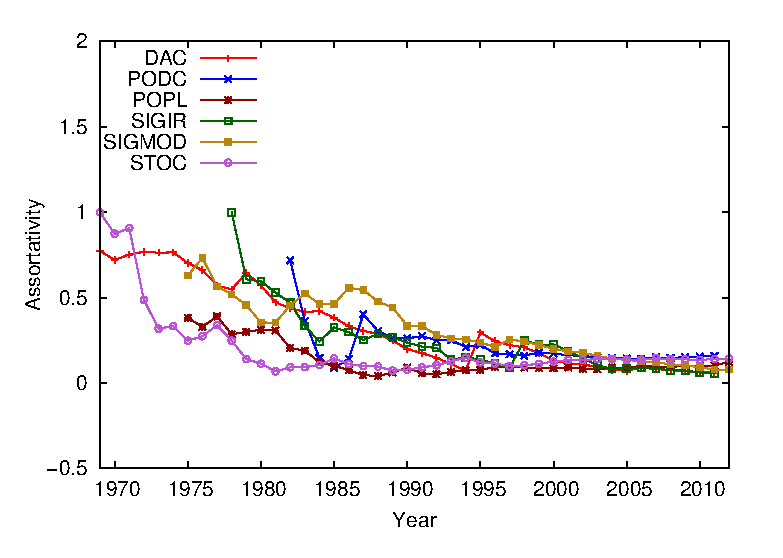
\includegraphics[scale=.33]{graficos/sigs_metricas_acumuladas_1_em_1_ano/assortatividade_grupo_temporal_web.eps}
  }%
  \subfigure[Average shortest path]{%
    \label{fig:average_shortest_path_1_in_1}
    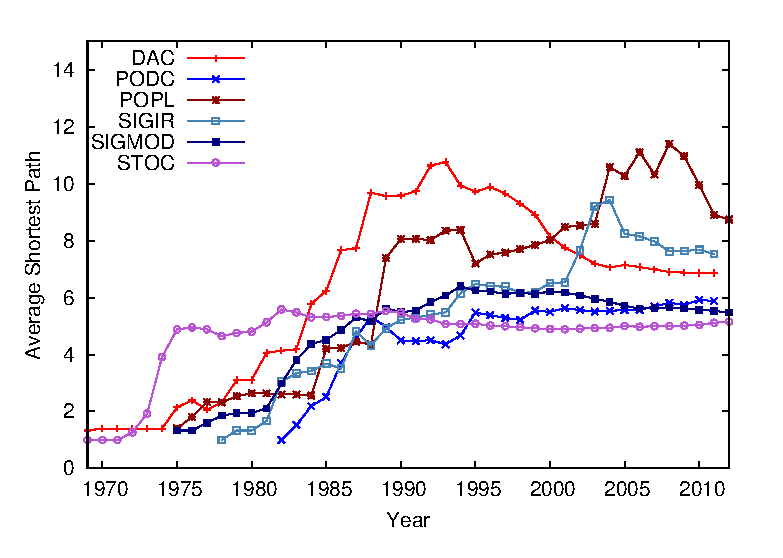
\includegraphics[scale=.33]{graficos/sigs_metricas_acumuladas_1_em_1_ano/caminho_minimo_medio_grupo_temporal_web.eps}
  }%
  \\
  \subfigure[Clustering coefficient]{%
    \label{fig:clustering_coefficient_1_in_1}
    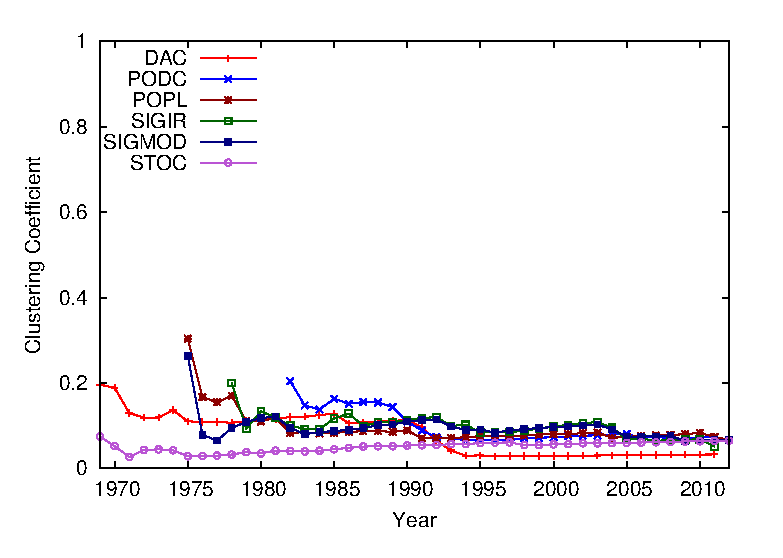
\includegraphics[scale=.33]{graficos/sigs_metricas_acumuladas_1_em_1_ano/coeficiente_agrupamento_grupo_temporal_web.eps}
  }%
  \subfigure[Largest connected component]{%
    \label{fig:largest_connected_component_1_in_1}
    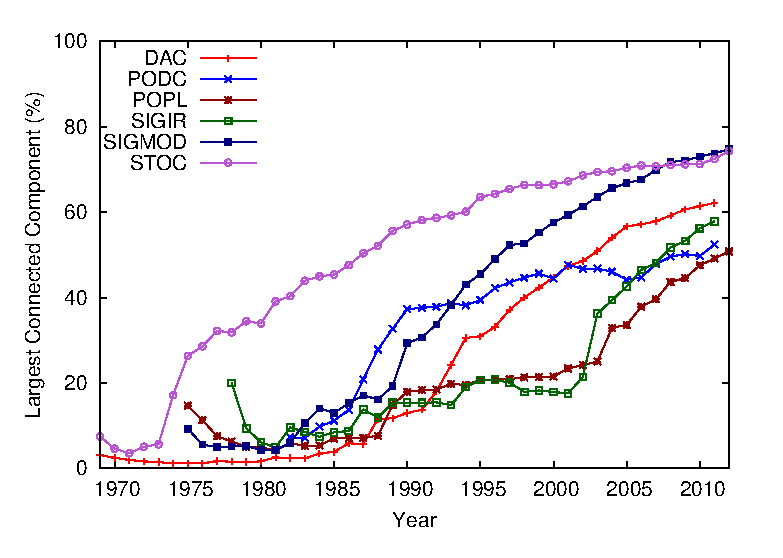
\includegraphics[scale=.33]{graficos/sigs_metricas_acumuladas_1_em_1_ano/porcentagem_maior_componente_grupo_temporal_web.eps}
  }%
  \end{center}
  \caption{Metrics accumulated from 1 in 1 year}
  \label{fig:metrics_accumulated_1_in_1}
\end{figure}

%\begin{figure*}
%\centering
%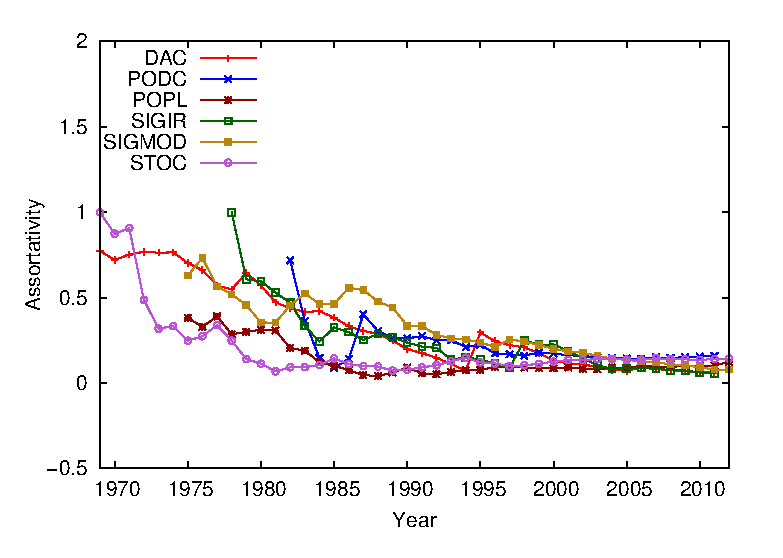
\includegraphics[scale=.4]{graficos/sigs_metricas_acumuladas_1_em_1_ano/assortatividade_grupo_temporal_web.eps}
%\caption{Assortativity accumulated from 1 in 1 year}
%\label{fig:assortativity_1_in_1}
%\end{figure*}

%\begin{figure*}
%\centering
%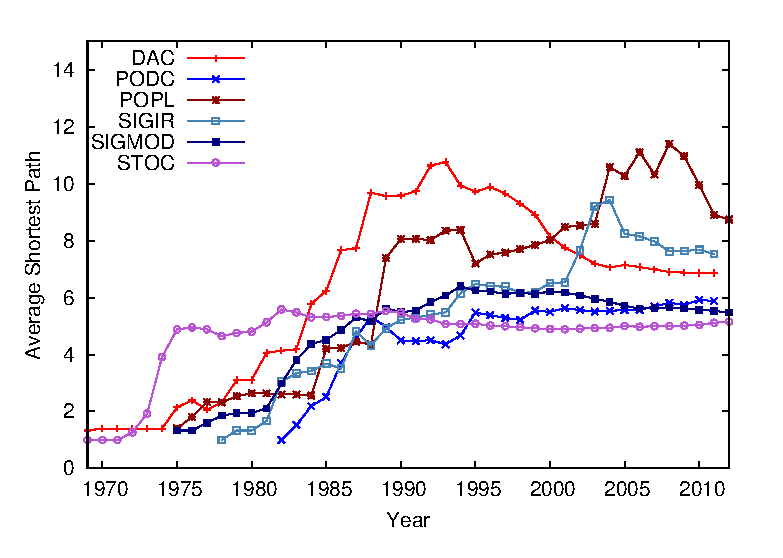
\includegraphics[scale=.4]{graficos/sigs_metricas_acumuladas_1_em_1_ano/caminho_minimo_medio_grupo_temporal_web.eps}
%\caption{Average shortest path accumulated from 1 in 1 year}
%\label{fig:average_shortest_path_1_in_1}
%\end{figure*}

%\begin{figure*}
%\centering
%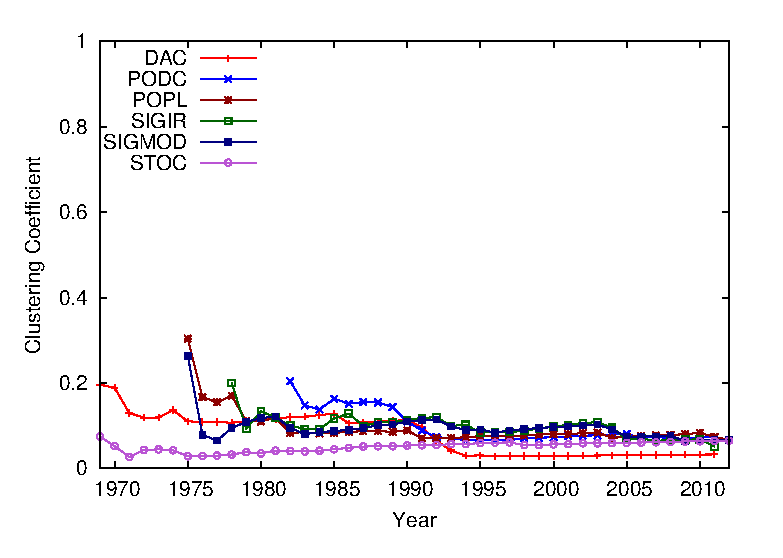
\includegraphics[scale=.4]{graficos/sigs_metricas_acumuladas_1_em_1_ano/coeficiente_agrupamento_grupo_temporal_web.eps}
%\caption{Clustering Coefficient accumulated from 1 in 1 year}
%\label{fig:clustering_coefficient_1_in_1}
%\end{figure*}

%\begin{figure*}
%\centering
%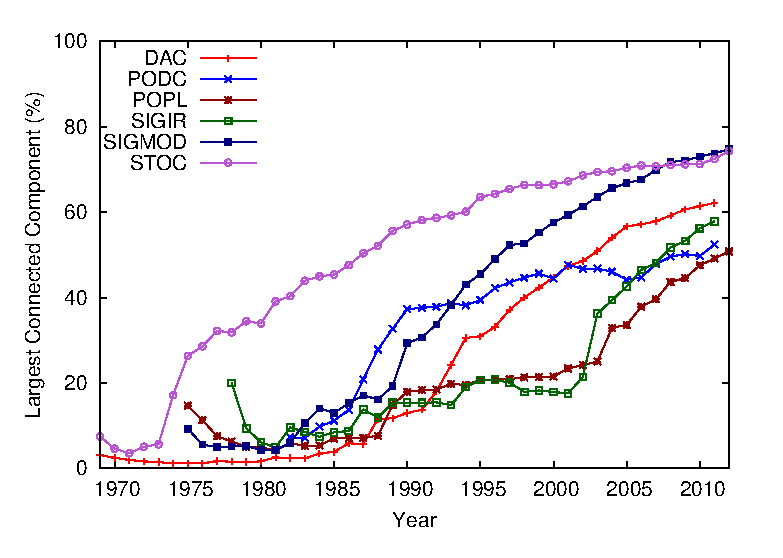
\includegraphics[scale=.4]{graficos/sigs_metricas_acumuladas_1_em_1_ano/porcentagem_maior_componente_grupo_temporal_web.eps}
%\caption{Largest connected component accumulated from 1 in 1 year}
%\label{fig:largest_connected_component_1_in_1}
%\end{figure*}

\section{Defining Community Core}

\subsection{Quantifying authors involvement}
% {\bf Desirable:\\
%      \sout{-Rank better prolific authors (h-index)} \\
%      \sout{-Frequent involvement (numero de papers}) \\
%      \sout{-Recent involvement (janela temporal)}}\\\\
In the academic community, the researchers are always seeking to contribute for yours areas, such contributions occurs
through publications, it is importants a mechanism to measures the impact of a researchers inside of the community. 
For this, there is a measures called of h-index \cite{Hirsch:2005}, the h-index is based on the number of publications 
and its references to a particular author has. This measure is widely accepted by the academic community.\\
The h-index is a metric created to measure how prolific a researcher is, but it alone is not sufficient to quantify
the importance of a researcher in a particular community, as a conference. To measure the impact of a
researcher in a conference, we must consider your contributions to the community in general, in this case, h-index, 
and your contributions to a specific community.
It is important consider the contributions to a specific community, because two researcher can have the same h-index. That
does not mean that both have the same importance for the conference, because one can have more publications at a conference 
the other. We define the number of publications of a researcher in a given conference as the measure that quantifies 
their involvement in a given communities.\\
Here, we have two measure, the h-index measure the researcher importance in the academic community and the number of 
publications that measure the importance of a researcher in a specific community. But without a temporal information,
it is only possible define how importante the researcher was to the entire community, because we should use the data 
accumulated over the years. So, we need aggregate the temporal information in our measure, we need consider the number 
of publications of a researcher in a given time \textit{t}.\\
After these definitions, it is possible to determine a measure to rank the researcher according to their importance
to a community at a given time, where the can be a temporal window. We define this measure as core score and can be see
in the Equation \ref{eq:core_score}.
\begin{equation} 
  \label{eq:core_score}
  Core{ }Score[a] = h\textrm{-}index[a] * number\textrm{ }of\textrm{ }publication[a,t]
\end{equation}
where \textit{h-index[a]} represents the h-index of a given author and the \textit{number of publication[a,t]} represents 
the number of publications of a given author in a given time.

% The core score measures the author's importance of a given conference. The core score uses the publication number 
% of an author in a conference in the time \textit{t} and their h-index \cite{Hirsch:2005}. The h-index, defined 
% as the number of papers with citations number higher or equal to \textit{h}, it is a useful index to characterize 
% the scientific output of a researcher. The core score is defined as:
% \begin{equation}Core Score = h\textrm{-}index * number\textrm{ }of\textrm{ }publication[t]\end{equation}
% where h-index is computed using the data of shine and the number of publication in the time \textit{t} is computed 
% using the data of DBLP\cite{Ley:2009}.

\subsection{Inferring authors h-index}
% {\bf-Por que nao google citations ou MS? \\
%      -Shine \\
%      -Correlacao com h-index do google}\\\\
As explained in the previous section, the h-index is measure accepts by the academic communities. The values of h-index 
can be found out in many tools of academic area as Google Scholar Citations\footnote{http://scholar.google.com/citations}, 
Microsoft Academic Search\footnote{http://academic.research.microsoft.com/} and others.\\
The h-index allows determine how prolific a researcher is, thus this information is a important point for this work.
At first we tried to use the data from Google Scholar Citations, but we had basically two problems which hampered this.
This tool does not have a API to crawl the data, so this make the work hard, but what did we change
the direction to use this data, it is because not all researchers have a profile. Despite the Google Scholar Citations 
has values acceptable to h-index in the academic community, for it to calculate the researchers' h-index, they need create 
a profile providing personal data. In our crawl, it only found out 30\% of researcher of DBLP in Google Scholar Citations,
thus one amount as low could bias this work.\\
We also try to use the Microsoft Academic Search, that differently of Google Scholar Citations, it creates the researcher 
profile automatically, but it has lower values of h-index. The Microsoft Academic Search has an API to crawl the data, 
but this API is basead on publications, which also hinders the crawl of researcher. When we send a query to the API, 
based in researcher name, the API return all publications that have that researcher as author. It is possible change 
the return to authors, but in this case, the API return all researchers that have at least one publication along 
with the researcher name entered.\\
Since the limitation of these tools, we decided to perform the calculation of the h-index using data from the 
SHINE project\footnote{http://shine.icomp.ufam.edu.br/}. The project collected many publications along with their 
references, they used this data to infer the h-index of academics conferences, as shown in the Table \ref{tab:sigs_conference_period}.
They collected the main conferences of each area of academic ... {\bf falar mais do shine}.\\
We crossed the data from the SHINE with DBLP and after this we have a number of citations of each publication, so we calculated
the h-index of each researcher. To validate this calcule, we selected, randomly, 10 researcher of each conference into Table
\ref{tab:sigs_conference_period} and crawled your profile in Google Scholar Citations. We obtain a value of 0.85 of 
pearson coefficient which indicates a strongly positive correlation, as can be seen in Figure \ref{fig:hindex_scatter_plot}.
\begin{figure}[!htb]
\centering
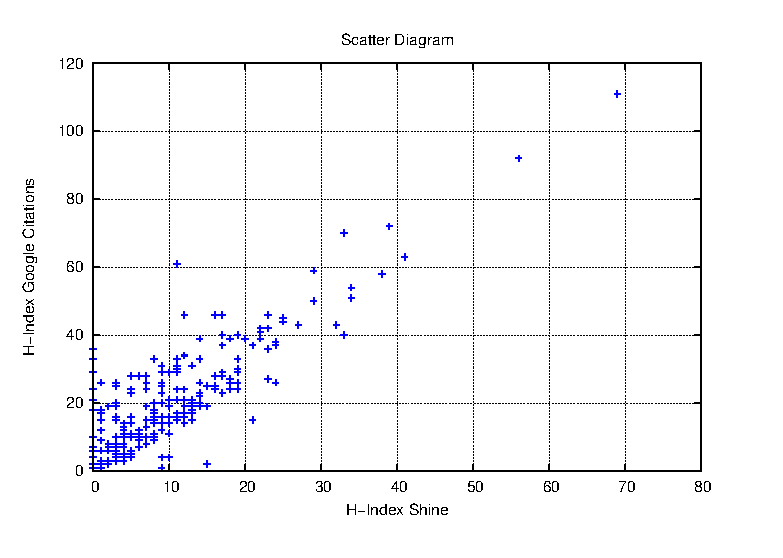
\includegraphics[scale=.5]{../dissertacao/graficos/hindex_scatter_plot.eps}
\caption{Correlation between H-Index infered and Google Scholar Citations }
\label{fig:hindex_scatter_plot}
\end{figure}

\subsection{Setting core size and time thresholds}
This work has a temporal focus, so to represent this issue we are using temporal sliding windows over the years. Several
experiments were performed varying the window size. Initially we varied the size between 1 and 5 years, but along with the
classic social network metrics and size variation of the Core Community, we would have many experiments in the study.
So, we need to determine two values, the size of the sliding window and the size of the core community.\\
To determine the size of the temporal window we calculate measure resemblance defined in \cite{Viswanath:2009} for all conferences.
We vary the values of the size window, between 1 and 5 years, and the size of core community, between
10\% and 60\%, so we plot the data where the x-axis represents the variation in the size of windows and the y-axis represents
the average values of resemblance, each line the variation of the size of the core community. The 
Figure \ref{fig:averange_values_resemblance} showns the behavior of the curves of conferences SIGMOD and SIGDOC. Again, due to lack 
of space, we are showing only this conferences, we choose them because they are the conferences with the highest h-index 
and the lowest, consecutively.
\begin{figure}[!htb]
  \begin{center}
    \subfigure[SIGMOD]{%
      \label{fig:sigmod_slide_window_top_list}
      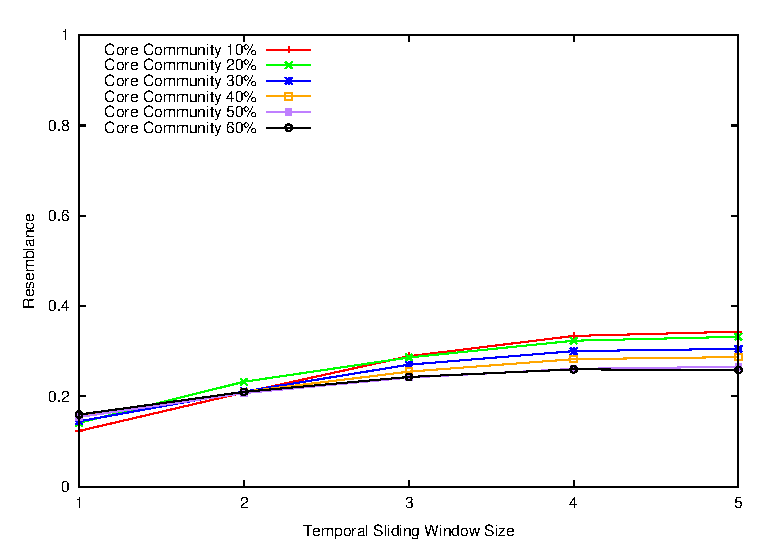
\includegraphics[scale=.33]{graficos/window_core_size/sigmod_slide_window_top_list.eps}
    }%
    \subfigure[SIGDOC]{%
      \label{fig:sigdoc_slide_window_top_list}
      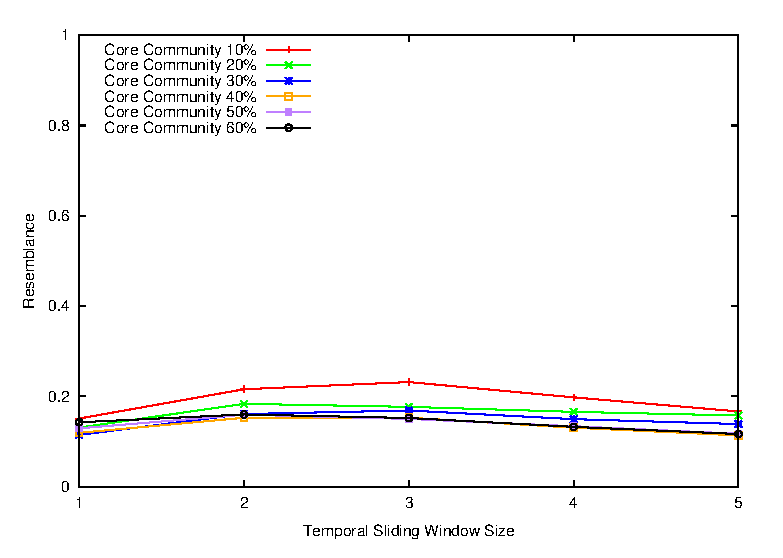
\includegraphics[scale=.33]{graficos/window_core_size/sigdoc_slide_window_top_list.eps}
    }%
  \end{center}
\caption{Average of the values of resemblance}
 \label{fig:averange_values_resemblance}
\end{figure}
How we can see in the Figure \ref{fig:averange_values_resemblance}, the behavior of the curves are similar, so we use the
angular coefficient to calculate the slope of the curves and after we compute the average of the value. The window size
3 is, in most cases, where the curve stabilizes, so it is the value adopted in this work. As for the size of Core 
Community, we adopted the value of 10\%, for the other experiments, due the proximity of the curves.


% {\bf-Descrever que foi escolhido janela de tamanho 3 utilizando coeficiente angular e core community
% de 10\% devido a proximidade das curvas.\\
% -Colocar grafico de media de resemblance do sigmod\\
% -Falar que as janelas foi feito o calculo da inclinacao da reta e a media das conferencias\\}

\subsection{Validations}
The measure defined as Core Score is important to shows the impact of the research in given community. We chosen two importants 
researchers to exemplify the use of the meausre. In the Figure \ref{fig:cc_kleinberg} is showns the impact of Jon Kleinberg in
conferences which he published. It is possible to see that he becomes relevant even in conferences that he is not part of
Core Community, because he is always ranked well. Similarly, we can see in the Figure \ref{fig:cc_luis_von_ahn} the impact
of Luis von Ahn, another important researcher in his area. This researcher is different from Jon Kleinberg, because he has a
considerable impact, however, he become part of Core Community only a conference and a short period, getting close to the Core
Community in subsequent periods. Importantly, we are showing only the conferences listed in Table \ref{tab:sigs_conference_period}.\\
\begin{figure}[!htb]
  \begin{center}
    \subfigure[Jon Kleinberg]{%
      \label{fig:cc_kleinberg}
      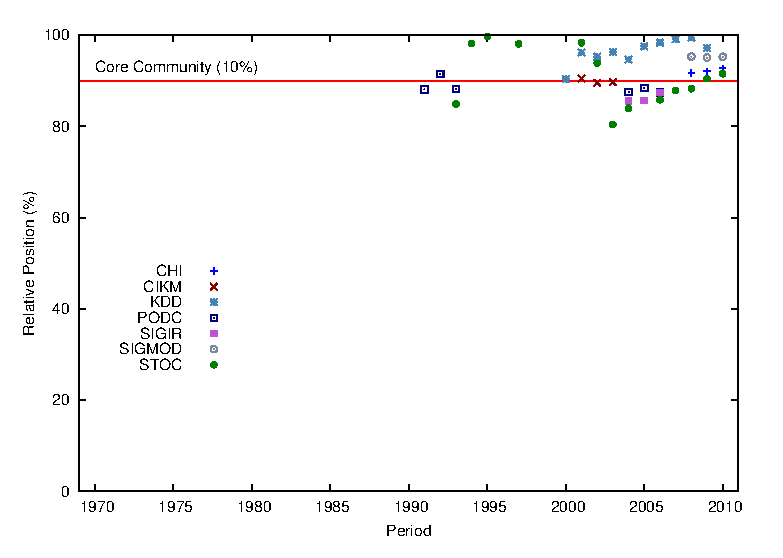
\includegraphics[scale=.33]{graficos/validacao_core_community/cc_kleinberg.eps}
    }%
    \subfigure[Luis von Ahn]{%
      \label{fig:cc_luis_von_ahn}
      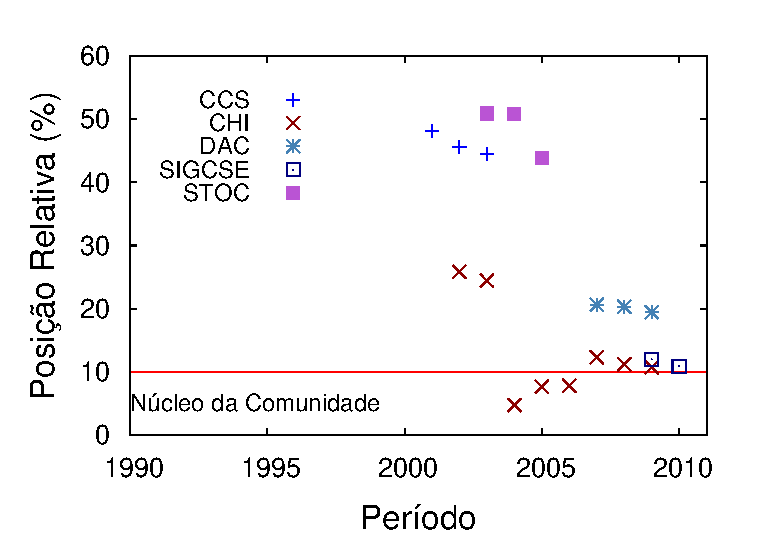
\includegraphics[scale=.33]{graficos/validacao_core_community/cc_luis_von_ahn.eps}
    }%
  \end{center}
\caption{Ranking using Core Score}
 \label{fig:rank_core_score_authors}
\end{figure}
This way, we showed the impact of the two research in the conferences, but who are the researchers who appear most often in the
Core Community of each communities, or in this case, conferences? In the Table \ref{tab:authors_frequency_core_community} is 
shown that main confereces linked the web area, it is possible to see the researchers known by the academic community.
\begin{table*}[!htb]
\centering
\caption{The researchers who appear most often in the Core Community over the years.}
\label{tab:authors_frequency_core_community}
{\small
\begin{tabular}{|c|l|l|l|l|} \hline
 & CIKM & KDD & SIGIR & SIGMOD\\ \hline
1\textordmasculine & Philip S. Yu & Heikki Mannila & W. Bruce Croft & David J. DeWitt\\ \hline
2\textordmasculine & Jiawei Han & Jiawei Han & Clement T. Yu & Michael Stonebraker\\ \hline
3\textordmasculine & Ling Liu & Eamonn J. Keogh & Susan T. Dumais & H. V. Jagadish\\ \hline
4\textordmasculine & Clement T. Yu & Martin Ester & James Allan & Rakesh Agrawal\\ \hline
5\textordmasculine & Christos Faloutsos & Bing Liu & Justin Zobel & Christos Faloutsos\\ \hline
6\textordmasculine & James Allan & Padhraic Smyth & Alistair Moffat & Raghu Ramakrishnan\\ \hline
7\textordmasculine & Elke A. Rundensteiner & Charu C. Aggarwal & Norbert Fuhr & Jiawei Han\\ \hline
8\textordmasculine & Ke Wang & Philip S. Yu & James P. Callan & Gerhard Weikum\\ \hline
9\textordmasculine & Amr El Abbadi & Ke Wang & Yiming Yang & Philip A. Bernstein\\ \hline
10\textordmasculine & W. Bruce Croft & Hans-Peter Kriegel & Edward A. Fox & Jeffrey F. Naughton\\ \hline
11\textordmasculine & Ming-Syan Chen & Rakesh Agrawal & Gerard Salton & Hector Garcia-Molina\\ \hline
12\textordmasculine & Divyakant Agrawal & Jian Pei & Ricardo A. Baeza-Yates & Michael J. Carey\\ \hline
13\textordmasculine & C. Lee Giles & Wynne Hsu & Jian-Yun Nie & Joseph M. Hellerstein\\ \hline
14\textordmasculine & Weiyi Meng & Qiang Yang & Mark Sanderson & Philip S. Yu\\ \hline
15\textordmasculine & Berthier A. Ribeiro-Neto & Christos Faloutsos & Charles L. A. Clarke & Divesh Srivastava\\ \hline
16\textordmasculine & M. Tamer \"Ozsu & Huan Liu & Chris Buckley & Michael J. Franklin\\ \hline
17\textordmasculine & ChengXiang Zhai & Mohammed Javeed Zaki & ChengXiang Zhai & Jennifer Widom\\ \hline
18\textordmasculine & Javed A. Aslam & Pedro Domingos & Alan F. Smeaton & Hans-Peter Kriegel\\ \hline
19\textordmasculine & Hans-Peter Kriegel & Jon M. Kleinberg & Zheng Chen & Hamid Pirahesh\\ \hline
20\textordmasculine & Bing Liu & Vipin Kumar & Ophir Frieder & Surajit Chaudhuri\\ \hline
\end{tabular}
}
\end{table*}

% {\bf%-Colocar calculo referente a posicao do kleinberg no core community nas conferencias \\
%     -Colocar autores que mais apareceram no core communities das conferencias com maior shine\\}

\section{Analisys of the communities core}

\subsection{New x Old communities}

\subsection{Conferences size}

\subsection{Impact of the core on the communities structure}
{\bf reproduzir trabalho do rich club \cite{Xu:2010}}

\begin{table*}[!htb]
\centering
\caption{Corelation between average core score of the core community and the metrics of complex networks}
\label{tab:correlation_metrics}
{\small
\begin{tabular}{|l|c|c|c|c|c|c|c|} \hline
Conference & Diameter & Ave. Short P. & Clus. Coef. & Assort. & Larg. Com. Con. & Ave. Deg. Node & Num. Nodes\\ \hline
CCS & 0,34 & 0,2 & 0,23 & -0,2 & 0,45 & 0,14 & -0,13\\ \hline
CHI & 0,75 & 0,79 & -0,62 & -0,74 & 0,76 & 0,77 & 0,58\\ \hline
CIKM & 0,56 & 0,56 & -0,52 & -0,67 & 0,39 & 0,87 & 0,64\\ \hline
DAC & 0,8 & 0,85 & -0,49 & -0,63 & 0,76 & 0,92 & 0,84\\ \hline
HSCC & 0,17 & 0,45 & -0,62 & -0,71 & 0,87 & 0,55 & -0,55\\ \hline
ICSE & 0,81 & 0,83 & -0,52 & -0,84 & 0,68 & 0,8 & 0,78\\ \hline
ISCA & 0,63 & 0,55 & 0,54 & -0,32 & 0,63 & 0,81 & 0,41\\ \hline
ISSAC & 0,05 & 0,01 & -0,25 & -0,43 & -0,07 & 0,21 & 0,78\\ \hline
KDD & 0,1 & 0,17 & -0,33 & -0,67 & 0,2 & 0,14 & 0,2\\ \hline
MICRO & 0,35 & 0,35 & 0,28 & -0,36 & 0,52 & 0,51 & 0,36\\ \hline
MOBICOM & -0,04 & 0,11 & 0,13 & -0,65 & 0,23 & -0,09 & 0,02\\ \hline
Multimedia & 0,67 & 0,68 & -0,91 & -0,95 & 0,67 & 0,69 & 0,75\\ \hline
PODC & 0,4 & 0,42 & -0,23 & -0,2 & 0,13 & 0,68 & 0,57\\ \hline
POPL & 0,21 & 0,2 & 0,23 & -0,43 & 0,25 & 0,19 & 0,05\\ \hline
SAC & 0,48 & 0,59 & 0,16 & -0,39 & -0,55 & 0,16 & 0,23\\ \hline
SIGCOMM & 0,18 & 0,19 & 0,05 & -0,81 & 0,49 & 0,41 & -0,03\\ \hline
SIGCSE & 0,88 & 0,84 & -0,22 & -0,5 & 0,93 & 0,87 & 0,8\\ \hline
SIGDOC & 0,73 & 0,78 & -0,36 & -0,89 & 0,66 & 0,76 & 0,05\\ \hline
SIGGRAPH & 0,79 & 0,85 & -0,45 & -0,75 & 0,94 & 0,88 & 0,55\\ \hline
SIGIR & 0,83 & 0,85 & -0,42 & -0,77 & 0,7 & 0,89 & 0,88\\ \hline
SIGMETRICS & 0,31 & 0,24 & 0,3 & -0,44 & 0,37 & 0,64 & 0,43\\ \hline
SIGMOD & 0,78 & 0,81 & 0,27 & -0,61 & 0,77 & 0,87 & 0,68\\ \hline
SIGUCCS & 0,38 & -0,22 & 0,53 & -0,13 & 0,51 & 0,7 & 0,57\\ \hline
STOC & 0,61 & 0,63 & 0,54 & -0,37 & 0,82 & 0,88 & 0,68\\ \hline
{\bf Average} & {\bf 0,49} & {\bf 0,49} & {\bf -0,11} & {\bf -0,56} & {\bf 0,5} & {\bf 0,59} & {\bf 0,42}\\ \hline
\end{tabular}
}
\end{table*}


\section{Conclusions}

\section{Future work}
-Ajustes na formula de Core Score:\\
-Computar h-index a todo momento, considerando o tempo t em analise\\
-Mudar a formula para considerar publicacoes feitas no passado, no entanto, colocar uma penalidade. (vida trabalho do peterson)\\
\\
-Realizar estudo semelhante em outra rede, tipo twitter, o h-index poderia ser alterado para um calculo de infuencia
%
%\section{Sugestões}
%Uma sugestão aqui nesse ponto é medir o número de shifts de comunidades em função do tamanho da janela para escolhermos um 
%tamanho de janela adequado, como fizemos anteriormente.\
%De posse dessa medição do core-score, vamos poder analisar o impacto nas caracteristicas estruturais das rede quando grandes 
%lideranças são perdidas. Será que as comunidades se renovam e mantém as propriedades ou não? 
%
% The following two commands are all you need in the
% initial runs of your .tex file to
% produce the bibliography for the citations in your paper.
\bibliographystyle{abbrv}
\bibliography{draft}  % sigproc.bib is the name of the Bibliography in this case
 
%\end{document}  % This is where a 'short' article might terminate
\end{document}
